\chapter{Mesh Shading}

% @TODO: Mention that this is rasterization pipeline!

Mesh Shaders were were first introduced to nVidia Touring GPUs in 2018 as a part of
"a new programmable geometric shading pipeline" and build upon the compute programming 
pipeline \cite[Christoph Kubisch]{Kubisch2018}. Therefore, they aim to optimize work by 
using the available hardware more efficiently. This section will break down the differences 
of the Mesh Shading Pipeline compared to the traditional Vertex Shading Pipeline. In order 
to evaluate these differences effectively, we will start by having a closer look at the 
Vertex Shading Pipeline.

\section{The Vertex Shading Pipeline}

The term \emph{Vertex Shading Pipeline} refers to the traditional rendering pipeline, which 
describes the different steps of the creation of a final output image, generated by the 
computer. Central to this pipeline are two GPU programs, called \emph{shaders}. The 
\emph{Vertex Shader} operates on the vertices of a given 3D model representation. 
The \emph{Pixel Shader} (also referred to as \emph{Fragment Shader}) operates on each pixel 
of the output frame buffer. Usually, the color values are calculated here, based on factors 
like light direction, camera position et cetera. \\

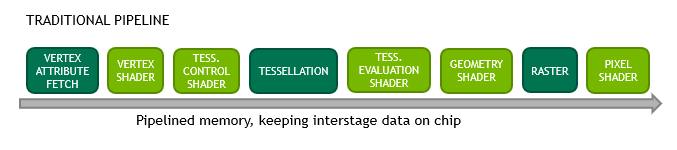
\includegraphics[width=\linewidth]{images/graphics/traditional-rendering-pipeline.png} % @TODO: Abbildungsverzeichnis

\noindent
The traditional rendering pipeline consists of several fix, programmable and optional steps.
Figure 5.1 shows these steps and their execution order. This pipeline represents more or less 
what the rendering pipeline has been for years up to this point. It is still used in most 
real time applications to this day, and even the mentioned Mesh Shading Pipeline relies on some of 
the central steps of this pipeline. 

% @TODO: Explain every step of the pipeline ? 

% @TODO: Show input and output data of the Vertex Shader

% @TODO: What do I wanna say here?

% Good or even better to show evolution of rendering? -> Vertex Shaded Immediate Rendering -> 
% Vertex Shaded Deferred Rendering -> Mesh Shaded Deferred Rendering ? 

\section{The Mesh Shading Pipeline}

% @TODO: Mesh Shading Rendering Pipeline

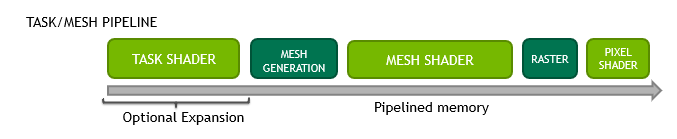
\includegraphics[width=\linewidth]{images/graphics/mesh-rendering-pipeline.png} % @TODO: Abbildungsverzeichnis

% @TODO: What are Mesh Shaders?


% @TODO: What are they good for?
% @TODO: How does the pipeline differ from the Vertex Shader Pipeline?

% @TODO: Meshlet Culling algorithm here or in 06_CaseStudy.tex?

\section{Differences and Comparison}

- Differences and performance benefits

% @TODO: Meshlet Creation
